\section{Introduction}

The project aims to model an epidemic with graph networks and to verify some theoretical results from well known papers in epidemiology. To model an epidemic, we will focus on the well known SIR model from Kermack and McKendrick \cite{Kermack700}, implementing a graph network and generating Monte Carlo simulation to check theoretical results built on SIR model. 
To check the different theoretical models from literature, we will use data from Flu epidemy in the United State during the 2016-2017 period.

Flu can be modelled only with one season because this epidemic occurs mainly during Winter (Figure 1).

\begin{figure}
    \centering
    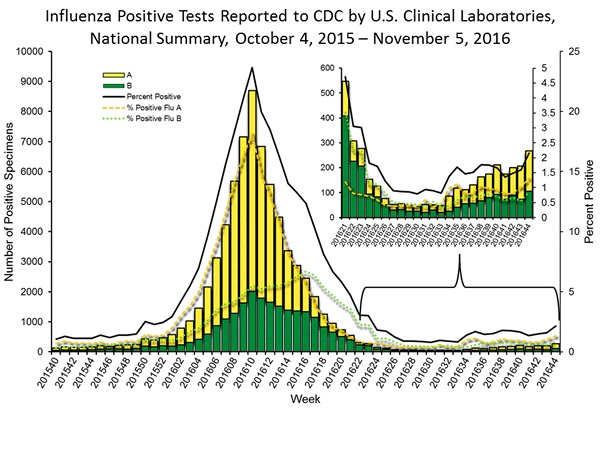
\includegraphics[scale=0.5]{WHONPHL44_small.jpg}
    \caption{Flu positive test over 2016-2017 in the U.S}
    \label{fig:my_label}
\end{figure}



\section{SIR Model}

The SIR model is a behavioral model in epidemiology and serve as a base mathematical framework of the main paper in this area. It helps understand complex dynamics of the spread of the disease.

The model splits the population into three categories: 
\begin{enumerate}
    \item Susceptible: (denoted by S). The number of people from the population susceptible to be ill. Thus, vaccinated people are not considered susceptible.
    \item Infected: (denoted by I). The number of people from the population infected.
    \item Recovered (denoted by R) The number of people from the population who have recovered and are now immune.
    
\end{enumerate}

The dynamics of these three variables over time can be expressed by the following differential equations:

$${\frac  {dS}{dt}}=-{\frac  {\beta IS}{N}}$$
$${\frac  {dI}{dt}}={\frac  {\beta IS}{N}}-\frac{I}{\lambda}$$
$${\frac  {dR}{dt}}=\frac{I}{\lambda}$$

$N$ is the number of people within the population. We assume that the population is constant over time because the dynamics of death and birth are often slower than the dynamics of Flu. Then:
$${\frac  {dS}{dt}}+{\frac  {dI}{dt}}+{\frac  {dR}{dt}}=0$$
$\beta$ is the incidence ratio. Then $\beta I S$ is the number of people who start out as susceptible and become infected during $dt$. We can express $\beta$ as the product between the number of people met during $dt$ times the probability that an infected person transmits the virus to someone else.


$\lambda$ is the average number of days a person is ill. Then $\frac{I}{\lambda}$ describes the flow to which the category "infected people" switch to the category "recovered people."


\section{Model of Flu epidemy with graph network}

Our goal is to test three models from literature and check if they are suitabled to model flu.

\subsection{Pastor-Satorras and Vespignani (2001) \cite{PhysRevLett.86.3200}}

First, the model follows an exponential distribution.
The first result from this paper is, when $\beta_{0} \Bar{k} \lambda s_0>1$, the network will converge to a steady state in which $I(t) > 0$. Then, we want to check if this result can be applied to our case of flu epidemy.

Second, the edge distribution follows a Power-law degree. ($P(k) ~ k^{-\nu}$

In the same way, we want to test if flu epidemy can be modelled by Power-law degree distribution.
Then, we want to apply the result from this paper to flu epidemy in the U.S.
Here, the authors show that:
\begin{itemize}
    \item for $2<\nu<3$ the network will converge to a steady state in which $I(t)>0$ for every set of parameter values.
    \item for $3<\nu$ the infection will be endemic in the network if and only if 
    $$\beta0 \lambda > \frac{\nu-1}{m \nu}$$
\end{itemize}


\subsection{Wang et al. and Ganesh et al., (2005) \cite{wang2003epidemic,ganesh2005effect}}

Here, the authors model the network as an arbitrary network.
The result from the paper is that $\beta \lambda < \frac{1}{\lamba_A}$, where $\lambda_A$ is the largest eigenvalue.


\subsection{Watts et al., 2005 \cite{watts2005multiscale}
}

The authors use a stochastic approach to model epidemics. We want to check if this approach is suited for our flu model in the U.S

\section{Data}

Our project data focus on flu epidemic in 2016-2017 in all U.S states.
 We have gathered data from the Centers for Disease Control and Prevention \footnote{https://www.cdc.gov/flu/}, which gathers weekly data from flu epidemic. These data are aggregated by state and by week.
 An interactive data visualization \footnote{https://gis.cdc.gov/grasp/fluview/fluportaldashboard.html} is also provided by the website.
 
 The most accurate data representing flu epidemic and the extent to which people are infected are the number of respiratory specimens tested (the entire population) and the number of people tested positive for influenza types A and B from this population.
 These data are collected by American laboratories\footnote{Exclusively WHO and NREVSS collaborating laboratories}
 
 Furthermore, we need the vaccinated ratio among our population. The Centers for Disease Control and Prevention gives this ratio on a weekly basis, by state and by age group.
 
 Finally, we have determined some parameters:
 \begin{itemize}
     \item $\lambda$ the number of days a people is ill is set to 2 weeks.
     \item $\beta$ is the product between the number of people met during $dt$ time the probability that an infected person transmits the virus to someone else. Then, the number of people met during $dt$ is $k$, the number of edges for one node in the graph. We set $p_inf$ at 0.6\footnote{explication}.

The last parameter to set is $\lambda$
 \end{itemize}



